\documentclass[12pt,a4paper]{scrartcl} 
\usepackage[utf8x]{inputenc}
\usepackage[english]{babel}
\usepackage{booktabs} % f\"ur Tabellen (Linien)
\usepackage{subfig}
\usepackage{graphicx} % f\"ur Bilder
\usepackage{import} % f\"ur pdf Bilder in einem anderen Ordner
\usepackage{cite} % für die Lit.bib
\usepackage{amssymb} % f\"ur Mathe Symbole
\usepackage{amsmath} % f\"ur Matrizen
\usepackage[usenames,dvipsnames]{xcolor} % f\"ur farbe
\usepackage{colortbl} % f\"ur farbige zeilen in tabellen
\usepackage{microtype} % bessere schriftsetzung f\"ur pdflatex
\usepackage{tikz}
\usepackage{notoccite} % "`richtige"' cite reihenfolge
\usepackage{chemfig} % paket für chemische Summen- und Strukturformeln
\usepackage{placeins}
\usepackage{float}
\usepackage{afterpage}
\usepackage{pdflscape}
\usepackage{hyperref}
\usepackage{changepage}

\usepackage{setspace} % Zeilenabstand
\onehalfspacing % 1.5x
\usepackage[inner=2cm,outer=2cm,top=2cm,bottom=2cm,includeheadfoot]{geometry} % Seitenr\"anderen
\parindent=0pt
\usepackage{multirow} % f\"ur spalten, die sich \"uber mehrere erstrecken
\usepackage{tabularx} % better table layout etc
\usepackage{subfig}
\usepackage{ngerman,setspace,fancyhdr}

\pagestyle{fancy}
\fancyhf{}
\chead{EVB-QMDFF Manual}
\newcommand{\CITE}{\textcolor{red}{[CITE]} }
%    Geometry of the pages: widths of borders
\usepackage{geometry}
\geometry{
  left=2.0cm,
  right=2.0cm,
  top=2.0cm,
  bottom=3cm,
%  bindingoffset=5mm
}


% recommendations for better float placement
\renewcommand{\topfraction}{.85}
\renewcommand{\bottomfraction}{.7}
\renewcommand{\textfraction}{.15}
\renewcommand{\floatpagefraction}{.66}
\renewcommand{\dbltopfraction}{.66}
\renewcommand{\dblfloatpagefraction}{.66}
\setcounter{topnumber}{9}
\setcounter{bottomnumber}{9}
\setcounter{totalnumber}{20}
\setcounter{dbltopnumber}{9}

\begin{document}
\begin{titlepage}
 \begin{adjustwidth}{0cm}{-1cm}

\begin{center}
\vspace{4cm} ~
\newline ~
\vspace{0.2cm}
\newline
\textbf{\LARGE EVB-QMDFF} \\[0.8cm]
\textbf{\Large RPMD and Rate Constant Calculations on Black-Box Potential Energy Surfaces}\\[1.3cm]


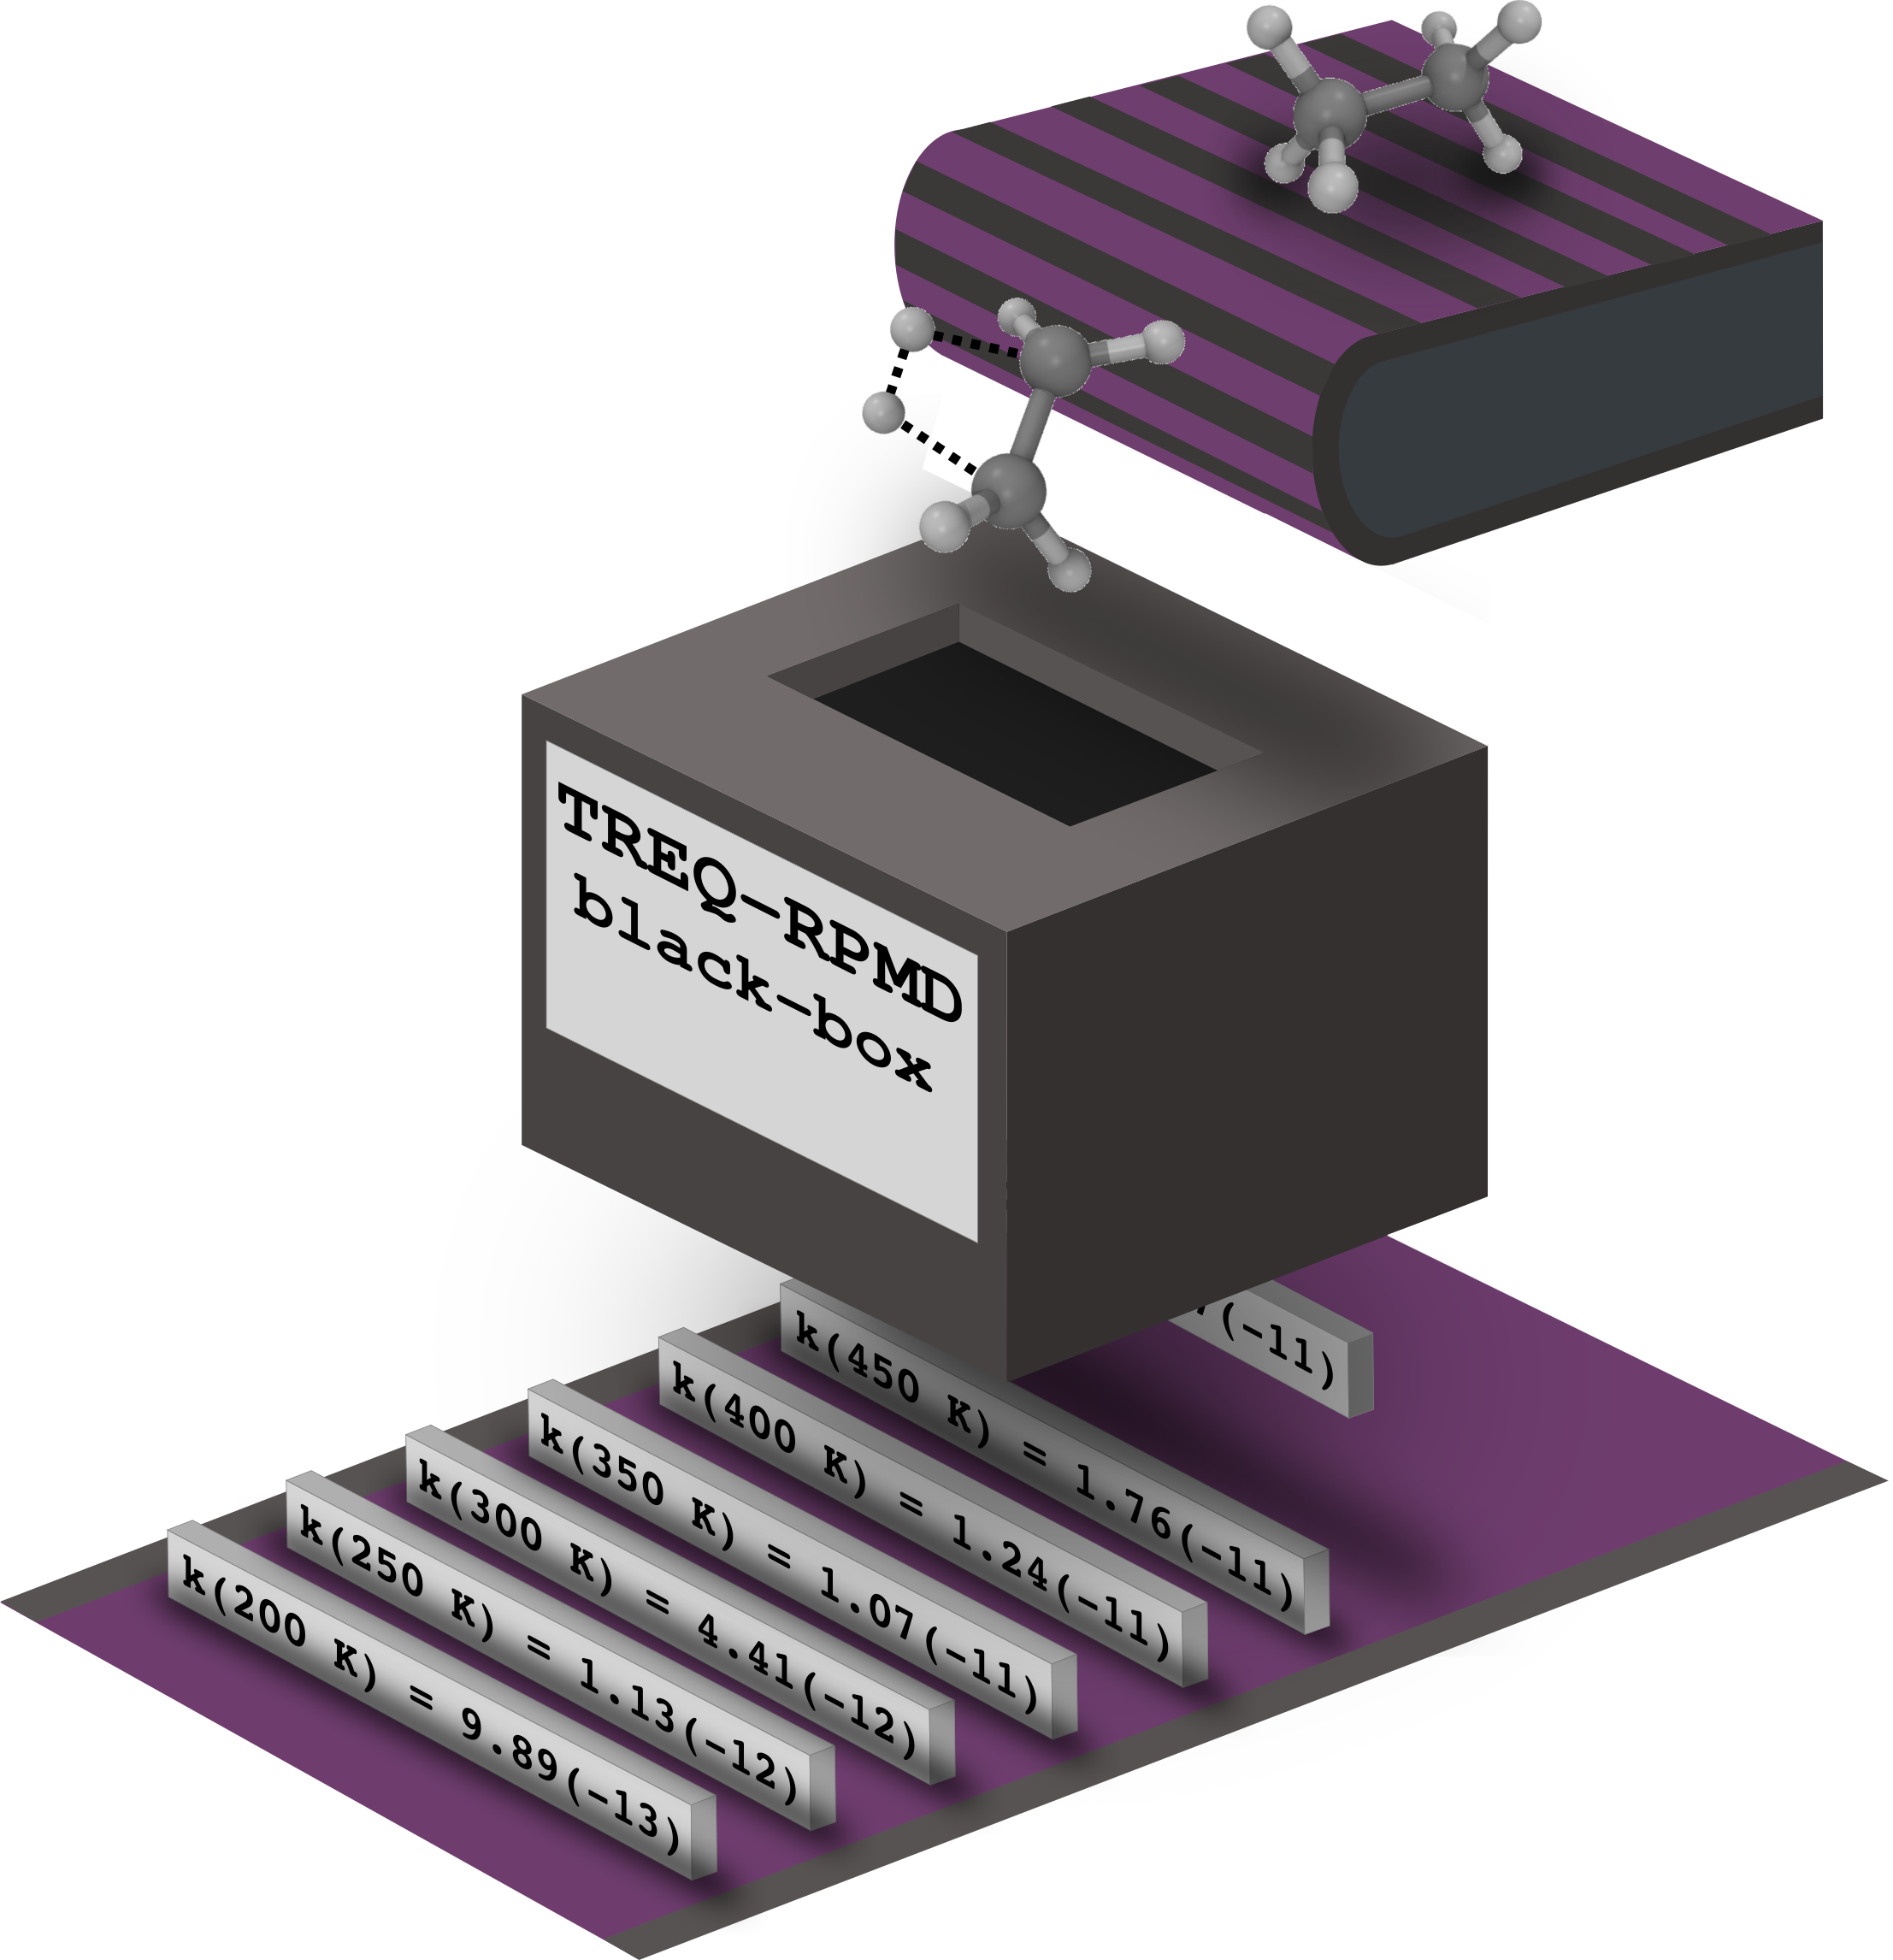
\includegraphics[width=0.56\textwidth]{figures/titlepic.png}



\vspace{1.3cm}

\textbf{\large{Julien Steffen}}

\vspace{1.3cm}
\textbf{\Large{Version 1.1, September 2021}}


\end{center}



\vfill
\end{adjustwidth}


\end{titlepage}

\tableofcontents

\newpage

\section{General Information}

EVB-QMDFF is a program package for molecular dynamics simulations.
It can both perform classical MD and ring polymer molecular dynamics (RPMD) on
potential energy surfaces built upon the quantum mechanically derived force field (QMDFF)
by \textsc{Grimme} and the empirical valence bond method by \textsc{Warshel} and others.

QMDFF is able to generate a fully-fledged potential energy description for an arbitrary
chemical system, leading to a reasonable description of the accessible energy
landscape as well as of bond breakings. With this ability, one can
e.g. simulate mechanochemical reaction with a single QMDFF.
Two or three QMDFF can be coupled via EVB in order to simulate arbitrary chemical elementary
reactions. Based on this simple idea, a list of EVB coupling methods, including
the newly-developed transition path corrected reaction path EVB-QMDFF (TREQ)
was implemented into the program package.
Based upon umbrella samplings of the reaction path, a protocol for black-box
calculations of chemical reaction rate constants was implemented, serving as a simple
and powerful tool for the calculation of those values.

A second branch is the simulation of liquid phases via QMDFF. It is possible to generate
a force field for a liquid of arbitrary composition from QMDFFs of the single components.
The targeted optimization of noncovalent QMDFF parameters is now possible as well,
leading to force fields of high quality for the liquid of interest, which can be sampled
via NVT or NpT dynamics classically or with RPMD.

EVB-QMDFF consists of a number of independent programs, serving to fulfill a number of
different tasks:

\begin{itemize}
 \item \textbf{qmdffgen}: Generates a QMDFF from given output of a QM calculation containing the
     bond orders, charges and frequencies of the reference structure.
 \item \textbf{evbopt}: Optimizes the parameters of a chosen EVB coupling term 
     (dE, dQ or DG coupling) for a chemical reaction
     based on two QMDFFs (reactand and product) and reference energies of the reaction path.
 \item \textbf{egrad}: Calculates energies and gradients for a given trajectory of structures
     with one of the given PES descriptions.
 \item \textbf{evb\_qmdff}: Performs geometry optimizations, gradient and frequency calculations of
     chemical systems with one of the given PES descriptions.
 \item \textbf{irc}: Optimizes the transition state and, starting from it, a reaction path with the
     IRC method.
 \item \textbf{dynamic}: Molecular dynamics simulations, both classical and RPMD, on QMDFF
    and EVB-QMDFF potential energy surfaces. Forces can be applied on different collective
    variables, for sampling of certain chemical processes.
 \item \textbf{rpmd}: Calculation of chemical reaction rate constants based on RPMD on EVB-QMDFF
     potential energy surfaces.
  \item \textbf{evb\_kt\_driver}: With a reaction path as input, reference calculations, PES setup
     with TREQ and RPMD samplings are done in black-box fashion, resulting in temperature-dependent
     reaction rate constants and Arrhenius parameters.
  \item \textbf{mult\_qmdff}: The QMDFF of a solvent box is built from given QMDFFs of single
     solvent molecules.
  \item \textbf{qmdffopt}: After automatic builtup of a suited trainset, 
     noncovalent QMDFF parameters can
     be optimized for better solvent properties.
\end{itemize}

\newpage

\section{Installation}

EVB-QMDFF consists of pure Fortran code and thus is quite easy to install.

\subsection{Prerequisites}

All you need is:

\begin{itemize}
 \item A Fortran compiler (\texttt{gfortran} or \texttt{ifort})
 \item \texttt{BLAS} and \texttt{LAPACK} linear algebra libraries
 \item \texttt{FFTW3} Fourier transform libraries 
 \item Some of the programs (\textbf{evbopt} and \textbf{rpmd}) can be run in parallel using MPI. 
 If you want to compile and run them in parallel, \texttt{MPI} must be installed.
\end{itemize}

\subsection{Settings}

After downloading EVB-QMDFF, go into the \texttt{EVB-QMDFF} main folder and open 
the \texttt{Makefile} located there.
In its header, the Fortran compilers (GNU or Intel) can be chosen:

\begin{verbatim}
#  Fortran compiler for serial version:
FC = gfortran  # GNU Fortran
# FC = ifort   # Intel Fortran compiler 
#  Fortran compiler for MPI version
# FC = mpif90  # GNU Fortran
# FC = mpifort # Intel Fortran compiler
\end{verbatim}

The serial GNU compiler is chosen as default, please uncomment your preferred version.

By default, the single program binaries are located both into the \texttt{bin} subdirectory 
of the program folder and the bin directory in your home (\texttt{~/bin}).
Plase edit this part right below the compiler settings to your preferred location:

\begin{verbatim}
 #  Location of the compiled and linked executables
BINDIR = ~/bin
\end{verbatim}


Now save the Makefile and copy it to the \texttt{src} subdirectory.

\subsection{Compilation}

In the \texttt{src} subdirectory, execute:

\begin{verbatim}
 make
\end{verbatim}

and the objects and executables will be compiled. 
Now, EVB-QMDFF is ready to use.


\newpage


\section{Program handling}

In this chapter, the handling of each program will be explained. For each of them, at least
one example is located into the \texttt{examples} folder of the EVB-QMDFF directory.
Switch to the subfolders named after the respective programs in order to calculate 
the examples prepared for you if you want to get more experienced in using EVB-QMDFF.

Besides the descriptions provided below, each program has a help function, that 
gives general information and a complete list of availabe keywords for handling.
It can be invoked with:

\begin{verbatim}
 [program.x] -h
\end{verbatim}

or 

\begin{verbatim}
 [program.x] -help
\end{verbatim}

For almost all programs, the main input file is a \texttt{[name].key} file, where all needed 
commands to execute your calculation are listed.

\subsection{qmdffgen}

\subsubsection{Introduction}

\textbf{qmdffgen} uses the output of an QM calculation for a molecule to generate a QMDFF for it.
This QMDFF is able to simulate the full configurational landscape of this molecule and further 
to describe bond breakings correctly.
A QMDFF needs a predefine set of information provided by the QM program:

\begin{itemize}
 \item Optimized geometry
 \item Wiberg-Mayer bond orders
 \item Hirshfeld charges 
 \item Hessian matrix
\end{itemize}

Provided the correct settings, all those can be obtained from a single QM calculation (see below).
After doing the QM calculation, qmdffgen can be invoked:

\begin{verbatim}
 qmdffgen.x
\end{verbatim}

The program is interative and asks you for the Software used for the reference calculation
(currently available: orca, Gaussian, Turbomole and CP2K), the number of QMDFFs to generate 
(one to three), and the prefix of the QM input files (name without file ending).
Then, the QMDFF is generated in a black-box procedure and directly useable for other calculations!

 
\subsubsection{Example 1: Octane with Orca} 

\textit{Folder}: \texttt{qmdff/ocane\_orca/} \newline

The input as well as the output of the QM reference calculation with orca is placed here.
Basically, the keywords for the reference calculation with orca are always the same.
Open the file \texttt{octane.inp}:

\begin{verbatim}
 ! PBE0 D3 def2-SVP opt freq
* xyz 0 1
C         -8.36972        0.54078       -0.36595
C         -6.84957        0.56234       -0.35222
...
H         -0.30022        5.11409        2.54651
H         -0.26113        4.29744        0.97442
*
%output
        Print[ P_Hirshfeld ] 1
end
\end{verbatim}

A geometry optimization of the octane molecule was done with the \texttt{PBE0} DFT functional
(with \texttt{Grimme} D3 dispersion correction) and the cheap \texttt{def2-SVP} basis set.
For useful output, a geometry optimization \texttt{opt} followed by a frequency calculation 
\texttt{freq} need to be done, further, the section

\begin{verbatim}
 %output
        Print[ P_Hirshfeld ] 1
end
\end{verbatim}

must be added for the calculation of Hirshfeld charges.
The \textbf{qmdffgen} program needs the \texttt{octane.hess} and \texttt{octane.out} files 
as reference. 

Since these are present, simply type 

\begin{verbatim}
 qmdffgen.x
\end{verbatim}


and give the respective commands during the interactive input.
Then, the QMDFF \texttt{octane.qmdff} will be generated.

During the calculation, the central quality parameters are printed into the terminal:

\begin{verbatim}
 Zero point vibr. energy comparison (FF/true, kcal)  :     150.432     154.650
 Mean absolute deviation (MAD) of frequencies (cm-1) :      54.560
\end{verbatim}

The MAD value in particular is a good indicator of the QMDFF-quality. It is calculated by 
performing frequency calculations for the QM reference and the QMDFF hessian and comparing 
them. Good QMDFFs achieve values between 20 and 50, if the value is above 100, something 
might went wrong during the QM reference calculation or the optimization.
If the error cannot be located, please let me know.
The QMDFF was written into \texttt{octane.qmdff}. This file is the entrypoint for 
all the other programs included into EVB-QMDFF.

A number of additional output files was produced during the QMDFF optimization.
these are:

\begin{itemize}
 \item \texttt{octane\_qmdff.log}: Detailed information about the QMDFF generation (QMDFF internal
      coordinates, fragments, Levenberg-Marquardt fit of the force constants and QMDFF quality).
      See the QMDFF paper \cite{qmdff} for more details about the whole procedure.
 \item \texttt{octane\_molden.out}: This file can be opened with the \texttt{molden} molecule 
      viewer in order to visualize the normal modes of the different frequencies of the 
      QMDFF hessian.
 \item \texttt{coord\_def.inp}: List of internal coordinates used to construct the QMDFF (bonds, 
      angles, dihedrals) in the formate also used for several other programs inside QMDFF
      (\textbf{irc}, \textbf{rpmd}, ...).
 \item \texttt{coord\_analysis.dat}: Values of all internal coordinates, of the Wilson matrix for 
      transformation of cartesian gradients into intenal coordinates and the Wilson matrix 
      derivative for the transformation of cartesian Hessians into internal coordinates. 
      These matrices are used for setup of the DG-EVB coupling term in \textbf{evbopt}.
\end{itemize}

\subsubsection{Example 2: Guaicol with Gaussian} 

\textit{Folder}: \texttt{qmdff/guaicol\_gaussian/} \newline

For Gaussian, geometry optimization and frequency calculation must be done separately, 
since a combined geopt+freq calculation writes out the Hessian in an incomplete formate.Therefore, the file \texttt{guaicol\_opt.gjf} performs the geometry optimization 
and the file \texttt{guaicol\_freq.gjf} performs the calculation of the Hessian.

The QMDFF can again be calculated by generated by typing:

\begin{verbatim}
 qmdffgen.x
\end{verbatim}

Note, that the prefix of the QM reference must be that of the frequency calculation, i.e.,
\texttt{guaicol\_freq}. 

The quality of the generated QMDFF can be seen from the lines:

\begin{verbatim}
  Zero point vibr. energy comparison (FF/true, kcal)  :      85.684      86.016
 Mean absolute deviation (MAD) of frequencies (cm-1) :      26.815
\end{verbatim}

The MAD value of 26 suggests a good description of the low-energy part of the 
potential energy surface of Guaicol with the generated QMDFF (which was written 
to \texttt{guaicol\_freq.qmdff}. 
The other output files are the same as explained in the first example. 

\subsection{evbopt}

\subsubsection{Introduction}

This program generates and optimizes the parameters of EVB coupling terms.
The coupling smoothly connects two QMDFFs, therefore these need to be present (generated with
\textbf{qmdffgen}) when an EVB coupling term is optimized.
In addition, some reference data describing the reaction must be present, serving as the 
training set for the optimization routine. The xyz-coordinates of the structures and the 
respective reference energies in a linewise format must be present.
Usually, a reaction path, generated from a NEB or IRC calculation, would be used for this.
For the RP-EVB and the related TREQ method, a reaction path is mandatory.

\subsubsection{dE-EVB}

\textit{Folder}: \texttt{evbopt/dE-EVB/} \newline

The simplest EVB coupling version is the energy-gap (dE)-EVB coupling.
Here, the off-diagonal coupling term depends only on the energetic distances of both
QMDFFs at the current coordinates ($C(\Delta E$).
A bunch of different functions depending on $\Delta E$ can be used, the easiest are
the constant coupling $C=a$ with no $\Delta E$-dependence at all and the \texttt{1g} 
coupling $C(\Delta E)=a \exp\left(-b (\Delta E)^2\right)$ with a Gaussian shape.

The main input file is the \texttt{evbopt\_de\_1g.key} file, where all essentially all
control parameters are listed:

\begin{verbatim}

FFNAME  min1.qmdff  min2.qmdff
 2EVB       -272.22659664700754     -272.16798367875066
 path_energies ref.dat
 path_structure struc.xyz
 coupling  sd2
 shift_manual
\end{verbatim}




\end{document}


